\rhead{ALE METHOD}

Fluid-structure interaction (FSI) problems play a crucial role in many engineering applications, particularly in the nuclear industry, where internal components such as fuel rods and steam generator tubes are subjected to fluid-induced vibrations. These vibrations can lead to structural fatigue, wear, and, in extreme cases, the failure of critical components.


\chapter{The Arbitrary Lagrangian-Eulerian Method}
To determine the flow of a fluid, it is necessary to describe the kinematics of all its material particles throughout time. To do so, one can adopt either an Euler description of motion, in which a fluid particle is identified by its initial position, or a Lagrange description of motion, in which a fluid particle is identified by its instantaneous position. 
Both descriptions are totally equivalent, leading to different forms of the Navier-Stokes equations that can be discretized on a stationary mesh grid (Euler) or a mesh grid that follows the motion of the fluid particles (Lagrange). In both cases, the mesh grids do not account for the motion of the boundaries, which makes the numerical simulations of the related Navier-Stokes equations delicate. To overpass this problem, several approaches, such as the immersed boundary methods~\cite{puscas2015three, puscas2015time, puscas2015conservative}, or the Arbitrary Lagrangian-Eulerian (ALE) method~\cite{donea2004arbitrary, fourestey2004second, koobus2000computation} have been developed. Here, we rely on the ALE method.

\section{ALE kinematic description}
\lhead{The Arbitrary Lagrangian-Eulerian Method}

In the ALE approach, the fluid flow is computed in a domain that is deformed in order to follow the movement of the fluid-solid interface. It provides a hybrid description not associated with the fluid particles and the laboratory coordinates. We associate the description with a moving imaginary mesh that follows the fluid domain.  The motion of the ALE computational mesh is independent of the material motion, the approach treats the mesh as a frame that moves with the arbitrary velocity $\mathbf{v}_{ALE}$. In the Eulerian approach, this velocity is zero, whereas it is equal to the velocity of the fluid particles in the Lagrangian approach. But in the ALE method, this velocity is equal to neither zero nor the velocity of the fluid particles; it varies smoothly and arbitrarily between both of them.  This method is a Lagrangian description in zones and directions near solid, and Eulerian elsewhere. 
In the ALE kinematic description, neither the Lagrangian (material frame) configuration ${R}_{\mathbf{X}}$ 
(coordinates are denoted by $ \mathbf{X}$), nor Eulerian (spatial frame) configuration $R_{\mathbf{x}}$ 
(coordinates are denoted $ \mathbf{x} $) is taken as the reference. A third domain is consider, 
the referential configuration (ALE frame) $R_{\boldsymbol{\xi}}$ in which the reference coordinates 
(also called mixed coordinates) $\boldsymbol{\xi}$ allows the identification of the grid 
points~\cite{donea2004arbitrary}. 
\begin{figure}[ht!]
\begin{centering}
\begin{tikzpicture}[scale=0.7, axis/.style={thick,->}]
    \coordinate (O) at (-0.8, -0.8);
    \draw[axis] (O) -- +(0.5, 0) ;
    \draw[axis] (O) -- +(0, 0.5) ;
    \draw[axis] (O) -- +(-0.25, -0.5);
    \draw (0.6, 0.5) node[right] {$R_{\boldsymbol{\xi}}$};
    \draw (-0.8, -0.3) node[right] {$\boldsymbol{\xi}$};
    
    \draw[axis] (-5., -5.5) -- (-5., -5.) ;
    \draw[axis] (-5., -5.5) -- (-4.5, -5.5) ;
    \draw[axis] (-5., -5.5) -- (-5.25, -6) ;
    \draw (-4., -4.) node[right] {$R_{\mathbf{X}}$};
    \draw (-5.1, -5.1) node[right] {$\mathbf{X}$};
    
    \draw[axis] (3., -5.5) -- (3., -5.) ;
    \draw[axis] (3., -5.5) -- (3.5, -5.5) ;
    \draw[axis] (3., -5.5) -- (2.75, -6) ;
    \draw (4.5, -4.) node[right] {$R_{\mathbf{x}}$};
    \draw (3., -5.2) node[right] {$\mathbf{x}$};
    
    \coordinate (c) at (0,0);
    \coordinate (d) at (-4,-5);
    \coordinate (e) at (4,-5);
    \draw[rounded corners=1mm] (c) \irregularcircle{2cm}{1mm};
    \draw[rounded corners=1mm] (d) \irregularcircle{2cm}{1mm};  
    \draw[rounded corners=1mm] (e) \irregularcircle{2cm}{1mm}; 

    \draw[-stealth,thick] (2.1, 0)to[bend left](3.5, -3.);
    \node[fill=white]  at (-3.5,-1) {$\mathbf{\Psi}$};
    \draw[-stealth,thick] (-2.1, 0)to[bend right](-3.5, -3.);
    \node[fill=white]  at (3.8,-1.2) {$\mathbf{\Phi}$};
    \draw[-stealth,thick] (-2.1, -6)to[bend right](2.2, -6.);
    \node[fill=white]  at (0.,-7.4) {$\boldsymbol{\varphi}$};
    
\end{tikzpicture}
\par\end{centering}
\protect\caption{\label{fig:ALE_frame}  Lagrangian~$\mathbf{X}$, Eulerian~$\mathbf{x}$, ALE~$\boldsymbol{\xi}$ frame references and transformations relating them.}
\end{figure}

Fig.~\ref{fig:ALE_frame} illustrates this configurations and the transformations which relate them. The referential domain is mapped into the material domain by $\mathbf{\Psi}$ and into the spatial domain by $\mathbf{\Phi}$.
The mapping from the material domain to the referential domain, is representing by: 
\begin{equation}\label{eq:Psi}
\begin{aligned}
\mathbf{\Psi}^{-1}: R_{\mathbf{X}} \times \left[t_0, t_{end}\right[ & \longrightarrow  R_{\boldsymbol{\xi}} \times \left[t_0, t_{end}\right[, \\
 (\mathbf{X}, t) & \longmapsto  \mathbf{\Psi}^{-1} (\mathbf{X}, t) = (\boldsymbol{\xi}, t),
\end{aligned}
\end{equation}
and his gradient is: 
\begin{equation}
\frac{\partial \mathbf{\Psi}^{-1}}{\partial (\mathbf{X}, t)} =
\begin{pmatrix}
\dfrac{\partial \boldsymbol{\xi}}{\partial \mathbf{X}}  & \mathbf{v}_{ALE}\\
\\
\mathbf{0}^{\operatorname{T}} & {1}
\end{pmatrix}, 
\end{equation}
where $\mathbf{0}^{\operatorname{T}}$ is a null row-vector and the velocity $\mathbf{v}_{ALE}$ is defined as:
\begin{equation}
\mathbf{v}_{ALE}(\mathbf{X},t) =  \left.\dfrac{\partial \boldsymbol{\xi}}{\partial t}\right|_{\mathbf{X}}  (\mathbf{X},t),
\end{equation}
where the index in the partial derivatives indicates the variables that remain constant during the derivation. The Jacobian $J$  determinant: 
\begin{equation}
J (\mathbf{X},t) = \det \left(  \left.\dfrac{\partial \boldsymbol{\xi}}{\partial \mathbf{X}}\right|_{t} \right) (\mathbf{X},t),
\end{equation}
provides a link between the referential coordinates $\boldsymbol{\xi}$ and the material coordinates $\mathbf{X}$. It also relates the current volume element $dV$ in the reference frame and the associated volume element $dV_0$ in the initial configuration: 
\begin{equation}
d V (\boldsymbol{\xi}, t) = J (\mathbf{X}, t) dV_0(\boldsymbol{\xi}, t).
\end{equation}
The time rate of change of the Jacobien is given by~\cite{donea1982arbitrary}:
\begin{equation}\label{eq:jacobien_time_deriv}
\left.\dfrac{\partial J}{\partial t}\right|_{\mathbf{X}}  (\mathbf{X},t) = J (\mathbf{X},t) \nabla \cdot \mathbf{v}_{ALE} (\boldsymbol{\xi}, t ).
\end{equation}

\section{ALE form of governing equations}
In order to relate the time derivative in the material and referential domains, let a scalar physical quantity be described by $ f (\mathbf{X},t) $  in the material description and by $f^{*} (\boldsymbol{\xi}, t)$ in the referential domain. Using the mapping $\mathbf{\Psi}^{-1}$~(\ref{eq:Psi}), the transformation from 
the material  description $f$  of the scalar physical quantity to the referential description $f^{*}$ can be related as:
\begin{equation}
f(\mathbf{X},t) = f^{*}(\mathbf{\Psi}^{-1}(\mathbf{X},t), t) \quad \text{or}  \quad  f = f^* \circ \mathbf{\Psi}^{-1},
\end{equation}
and its gradient is given by: 
\begin{equation}
\dfrac{\partial f}{\partial (\mathbf{X},t) }(\mathbf{X},t) = \dfrac{\partial f^*}{\partial (\boldsymbol{\xi},t) }(\boldsymbol{\xi},t) \dfrac{\partial \mathbf{\Psi}^{-1}}{\partial (\mathbf{X},t) }(\mathbf{X},t),
\end{equation}
which is amenable to the matrix form: 
\begin{equation}
\begin{pmatrix} \dfrac{\partial f}{\partial \mathbf{X}}   \quad  \left.\dfrac{\partial f}{\partial t}\right|_{\mathbf{X}}\end{pmatrix}  = \begin{pmatrix} \dfrac{\partial f^*}{\partial \boldsymbol{\xi}}   \quad  \left.\dfrac{\partial f^*}{\partial t}\right|_{\boldsymbol{\xi}}\end{pmatrix} 
\begin{pmatrix}
\dfrac{\partial \boldsymbol{\xi}}{\partial \mathbf{X}}  & \mathbf{v}_{ALE}
\\
\\
\mathbf{0}^{\operatorname{T}} & {1}
\end{pmatrix}, 
\end{equation}
after block multiplication, it leads to the fundamental ALE relation between 
the material and the referential time derivatives:
\begin{equation}
\left.\dfrac{\partial f}{\partial t}\right|_{\mathbf{X}} (\mathbf{X},t) = \left.\dfrac{\partial f^*}{\partial t}\right|_{\boldsymbol{\xi}} (\boldsymbol{\xi},t) + \mathbf{v}_{ALE} \dfrac{\partial f^*}{\partial \boldsymbol{\xi}} (\boldsymbol{\xi},t)
\label{eq:time_deriv_transformation}
\end{equation}
Using the identity $ \nabla \cdot (f^* \otimes \mathbf{v}_{ALE}) = f^* \nabla \cdot \mathbf{v}_{ALE} + \mathbf{v}_{ALE} \nabla f^*$, equation~(\ref{eq:jacobien_time_deriv}) results is:
\begin{equation}
J  \nabla \cdot (f^* \otimes \mathbf{v}_{ALE}) =  f^*\left.\frac{\partial J}{ \partial t} \right|_{\boldsymbol{\xi}} +  J \mathbf{v}_{ALE} \cdot \nabla f^*.
\label{eq:time_deriv}
\end{equation}
Finally, from equation~(\ref{eq:time_deriv}), results:
\begin{equation}
\left.\frac{\partial (J  f)}{ \partial t} \right|_{\mathbf{X}}  (\mathbf{X},t) =  J(\mathbf{X},t) \left( \left.\frac{\partial f^*}{ \partial t}\right|_{\boldsymbol{\xi}} +  \nabla \cdot (f^* \otimes \mathbf{v}_{ALE}) \right) (\boldsymbol{\xi}, t ).
\label{eq:transformation}
\end{equation}
 
By applying~(\ref{eq:transformation}) to the Navier-Stokes equations, we obtain the local form of the Navier-Stokes equations in a reference frame moving at an arbitrary velocity $\mathbf{v}_{ALE}$:
\begin{equation}\label{eq:NS_ALE}
\left\{
\begin{aligned}
\left.\frac{\partial (J \mathbf{v})}{\partial t} \right|_{\mathbf{X}} (\mathbf{X},t) &=  J(\mathbf{X},t)  \left(\nu\Delta \mathbf{v}   - \nabla \cdot  \left( (\mathbf{v} - \mathbf{v}_{ALE}) \otimes \mathbf{v} \right)  - \dfrac{1}{\rho}\nabla p\right) (\boldsymbol{\xi}, t ), \\
\nabla \cdot   \mathbf{v} \, (\boldsymbol{\xi}, t ) &= 0.
\end{aligned}
\right.
\end{equation}
The ALE method gives a formulation of the Navier-Stokes equations in a conservative form with a modification of the transport velocity by the grid's velocity.
Furthermore, we can remark that both purely Lagrangian or Eulerian mesh description are contained in the ALE form as particular cases. Chosen $\mathbf{\Psi} = \textbf{\textit{I}}$ it implies $\mathbf{X} = \boldsymbol{\xi} $ and $\mathbf{v} = \mathbf{v}_{ALE}$ which results into a Lagrangian description; the Eulerian  description corresponds to $\mathbf{\Phi} = \textbf{\textit{I}}$ which is equivalent to $\mathbf{x} = \boldsymbol{\xi} $ and it implies $\mathbf{v}_{ALE} = \mathbf{0}$.

In the ALE framework, the choice of appropriate fluid mesh
velocity is important. This arbitrary mesh velocity keeps the movement of the meshes under control according to the physical problem, and it depends on the numerical simulations. In general, a new elasticity equation is solved. For moderate deformations, one can pose an auxiliary Laplace problem that is known as harmonic mesh motion~\cite{duarte2004arbitrary}:

\begin{equation}
  \left\{
\begin{aligned}
\Delta \mathbf{v}_{ALE} &= \mathbf{0} \;\;\;\;\; \text{in the fluid domain,}\\
\mathbf{v}_{ALE} &= \mathbf{v}_{S} \;\;\; \text{at a solid interface,}\\
\mathbf{v}_{ALE} &= \mathbf{0} \;\;\;\;\; \text{at a free surface,} 
\end{aligned}
\right.
\label{harmonic_mesh}
\end{equation}
from which the kinematics of the mesh grid is updated, i.e. ${\textbf{x}}^{new}={\textbf{x}}^{old} + \Delta t{\textbf{v}}_{ALE}$.

\rhead{ALE METHOD}
\section{Principle of the ALE numerical method}
\lhead{Principle of the ALE numerical method}
To determine the flow of a fluid, it is necessary to describe the kinematics of all its material particles throughout time. To do so, one can adopt either an Euler description of motion, in which a fluid particle is identified by its instantaneous position, or a Lagrange description of motion, in which a fluid particle is identified by its initial position. 
Both descriptions are totally equivalent, leading to different forms of the Navier-Stokes equations that can be discretized on a stationary mesh grid (Euler) or a mesh grid that follows the motion of the fluid particles (Lagrange). In both cases, the mesh grids do not account for the motion of the boundaries, which makes the numerical simulations of the related Navier-Stokes equations delicate. 

To overpass this problem, several approaches, such as the immersed boundary methods~\cite{puscas2015three, puscas2015time, puscas2015conservative}, or the Arbitrary Lagrangian-Eulerian (ALE) method~\cite{donea2004arbitrary, fourestey2004second, koobus2000computation} have been developed. 
In the ALE approach, a fluid particle is identified by its position relative to a frame moving with a nonuniform velocity ${\textbf{v}}_{ALE}$. In this new frame of reference, the Navier-Stokes equations write
\begin{subequations}\label{eq:NS_ALE2}
\begin{align}
\nabla \cdot   \textbf{v} &= 0, \\
\frac{\partial J {\textbf{v}}}{\partial t}  &=  J \left(\nu\Delta {\textbf{v}}   - \nabla \cdot  ( ({\textbf{v}} - {\textbf{v}}_{ALE}) \otimes {\textbf{v}} )  - \frac{1}{\rho}\nabla p\right),
\end{align}
\end{subequations}
with $J$ the Jacobian of the transformation between the ALE and the Lagrange descriptions. The ALE method is actually a hybrid description between the Euler and the Lagrange descriptions, both of them corresponding to the particular cases ${\textbf{v}}_{ALE}={\textbf{0}}$ and ${\textbf{v}}_{ALE}={\textbf{v}}_{particle}$, respectively. 

In the ALE framework, the choice of ${\textbf{v}}_{ALE}$ is arbitrary as long as the deformation of the mesh grid remains under control. For moderate deformations, ${\textbf{v}}_{ALE}$ is usually defined as the solution of an auxiliary Laplace problem, eq.~\eqref{harmonic_mesh},
from which the kinematics of the mesh grid is updated.

\rhead{Grid motion}
\chapter{Large scale grid motion for ALE}
\lhead{Large scale grid motion for ALE}

The ability of mesh motion techniques to handle large boundary displacements remains a significant limitation of conventional approaches. To address this challenge, the present work proposes a robust, flexible, and easy-to-implement strategy designed to extend ALE methods to their limits in the context of extreme mesh distortions.

The first step toward this objective involves replacing the traditional elliptic formulation with a hyperbolic one, enabling an explicit solution procedure that avoids the inversion of global systems. A proof of concept for this approach was presented in~\cite{leprevost_computationally_2023}, with a focus on evaluating its computational efficiency. The second step focuses on managing large-scale mesh distortions within this framework by flexibly incorporating fictitious material behavior through the external open-source \textbf{MGIS} interface (version 2.2, mgis-rliv-2.2-commit-21466c14, available at \url{https://github.com/thelfer/MFrontGenericInterfaceSupport}
; see \cite{helfer_mfrontgenericinterfacesupport_2020} for details) into \textbf{MFront}, an open-source material mechanics code generation tool (version TFEL-4.2.3, available at \url{https://github.com/thelfer/tfel}
, distributed under the GPL license; see \cite{helfer_introducing_2015} for details). This integration is a key feature of the proposed strategy, as it eliminates the need to introduce complex, application-specific material mechanics code, thereby preserving its modularity. For more details on this coupling and its implementation, see~\cite{faucher2024very}.

\section{Switching to a hyperbolic equation for the nonlinear grid problem}

In this new framework, the mesh motion is governed by a hyperbolic problem, which is mathematically equivalent to a wave propagation equation. The objective is to ensure that the grid’s behavior remains as close as possible to the quasi-static response obtained with the classical elliptic formulation, eq.~\eqref{harmonic_mesh}. Since the dynamic effects—such as waves and vibrations—associated with the hyperbolic equation are not of interest in this context, it is necessary to introduce significant damping to suppress any unwanted temporal oscillations in the mesh motion. To maintain computational efficiency, a simple damping model is adopted, involving a single multiplicative coefficient $d_g$. The resulting formulation for the grid motion is then given by:
\begin{equation}
\label{eq-final-grid-problem}
  \begin{array}{c}
    \displaystyle \rho_g \frac{\partial^2 \mathbf{u}_g}{\partial t^2}\left ( \mathbf{x}, t \right ) + d_g \frac{\partial \mathbf{u}_g}{\partial t}\left ( \mathbf{x}, t \right ) - \nabla \cdot \boldsymbol{\sigma}_g \left [ \mathbf{u}_g \left ( \mathbf{x}, t \right ) \right ] = 0, \forall \mathbf{x} \text{ in the fluid domain } \Omega_F (t), \\
    \mathbf{u}_g \left ( \mathbf{x}, t \right ) = \mathbf{u}_{imp} \left ( \mathbf{x}, t \right ) \text{ on } \Gamma_{lag}(t). \\
    \boldsymbol{\sigma}_g \left [ \mathbf{u}_g \left ( \mathbf{x}, t \right ) \right ] \cdot \mathbf{n} \left ( \mathbf{x}, t \right ) = 0  \text{ on } \partial \Omega_F (t) \setminus \Gamma_{lag}(t).
  \end{array}
\end{equation}

\section{Time and space discretization of the hyperbolic grid problem}

The first step is to discretize in time with an explicit scheme for the displacement. The \textit{central difference} scheme from the Newmark family \cite{newmark_method_1959} is chosen, for its simplicity and wide usage. It writes, between times $t^n$ and $t^{n+1}$:
\begin{equation}
 % \begin{aligned}
     \dot{\mathbf{u}}_g^{n+\frac{1}{2}}  = \dot{\mathbf{u}}_g^n + \frac{\Delta t}{2} \ddot{\mathbf{u}}_g^n, \quad 
     \mathbf{u}_g^{n+1}  = \mathbf{u}_g^n + \Delta t \dot{\mathbf{u}}_g^{n+\frac{1}{2}}, \quad
     \dot{\mathbf{u}}_g^{n+1}  = \dot{\mathbf{u}}_g^{n+\frac{1}{2}} + \frac{\Delta t}{2} \ddot{\mathbf{u}}_g^{n+1},
  %\end{aligned}
\end{equation}
\noindent with $\dot{\mathbf{u}}_g = \frac{\partial \mathbf{u}_g}{\partial t}$, $\ddot{\mathbf{u}}_g = \frac{\partial^2 \mathbf{u}_g}{\partial t^2}$, $\Delta t = t^{n+1}-t^n$,  $\mathbf{u}_g^n = \mathbf{u}_g (\mathbf{x}, t^n)$ and same for all the time derivatives and instants, and with $t^{n+\frac{1}{2}} = \dfrac{t^{n+1}-t^n}{2} = t^n + \dfrac{\Delta t}{2}$.

The explicit time integration of the hyperbolic problem~\eqref{eq-final-grid-problem} is characterized by its conditional stability to prevent the accumulation of truncation errors due to the explicit displacement prediction. This is a well-studied topic in the literature for structural dynamics, for instance, in \cite{belytschko_computational_1983} and the currently used stability condition, known as the \textit{Courant-Friedrichs-Lewy} (CFL) condition \cite{courant_partial_1967}, expresses as:
\begin{equation}
    \Delta t_g < \min_{i \in \text{mesh cells}} \frac{l_i}{c_i}
    \label{eq:CFL}
\end{equation}
with $l_i$ is the characteristic length of mesh cell $i$ (for instance the smallest edge length, the smallest height or the diameter of the inner circle), $c_i$ is the speed of sound in mesh cell $i$, depending on the material model, the index $g$ is used to distinguish the time-step used for the grid problem from the time-step used for the fluid problem of reference.

If the stable time step for the grid problem is larger than the stable time step of the fluid problem, the grid can be updated with the fluid stable time step. In many cases, however, the stable time step for the grid problem will be smaller than the stable time step for the fluid problem. Classical ratios are discussed, for instance, in~\cite{leprevost_computationally_2023} depending on the fluid regimes of interest, laminar or turbulent in particular. In this case, to avoid penalizing the computational performance by forcing a more frequent resolution of the fluid problem, a subcycling algorithm is implemented for the grid motion. 

The complete algorithm is given in Fig.~\ref{fig:algorithm}. The main loop for the transient solution of the Navier-Stokes equations is on the right, with the superscript $n$ for the time steps. The solution of the grid motion problem is detailed on the left, providing the grid displacement, yielding the Jacobian $J^{n+1}$, and the grid velocity $\mathbb{V}^{n+1}_{h,g}$ necessary for the solution of the ALE discrete Navier-Stokes equations at time $t^{n+1}$. The general case with subcycling of the grid problem is considered, and the intermediate grid states between $t^n$ and $t^{n+1}$ are identified as $\hat{\mathbb{U}}_g$, $\dot{\hat{\mathbb{U}}}_g$ and $\ddot{\hat{\mathbb{U}}}_g$, using the superscript $k$ for the inner subcycling iterations. 

\begin{figure}[H] %[here]
\centering
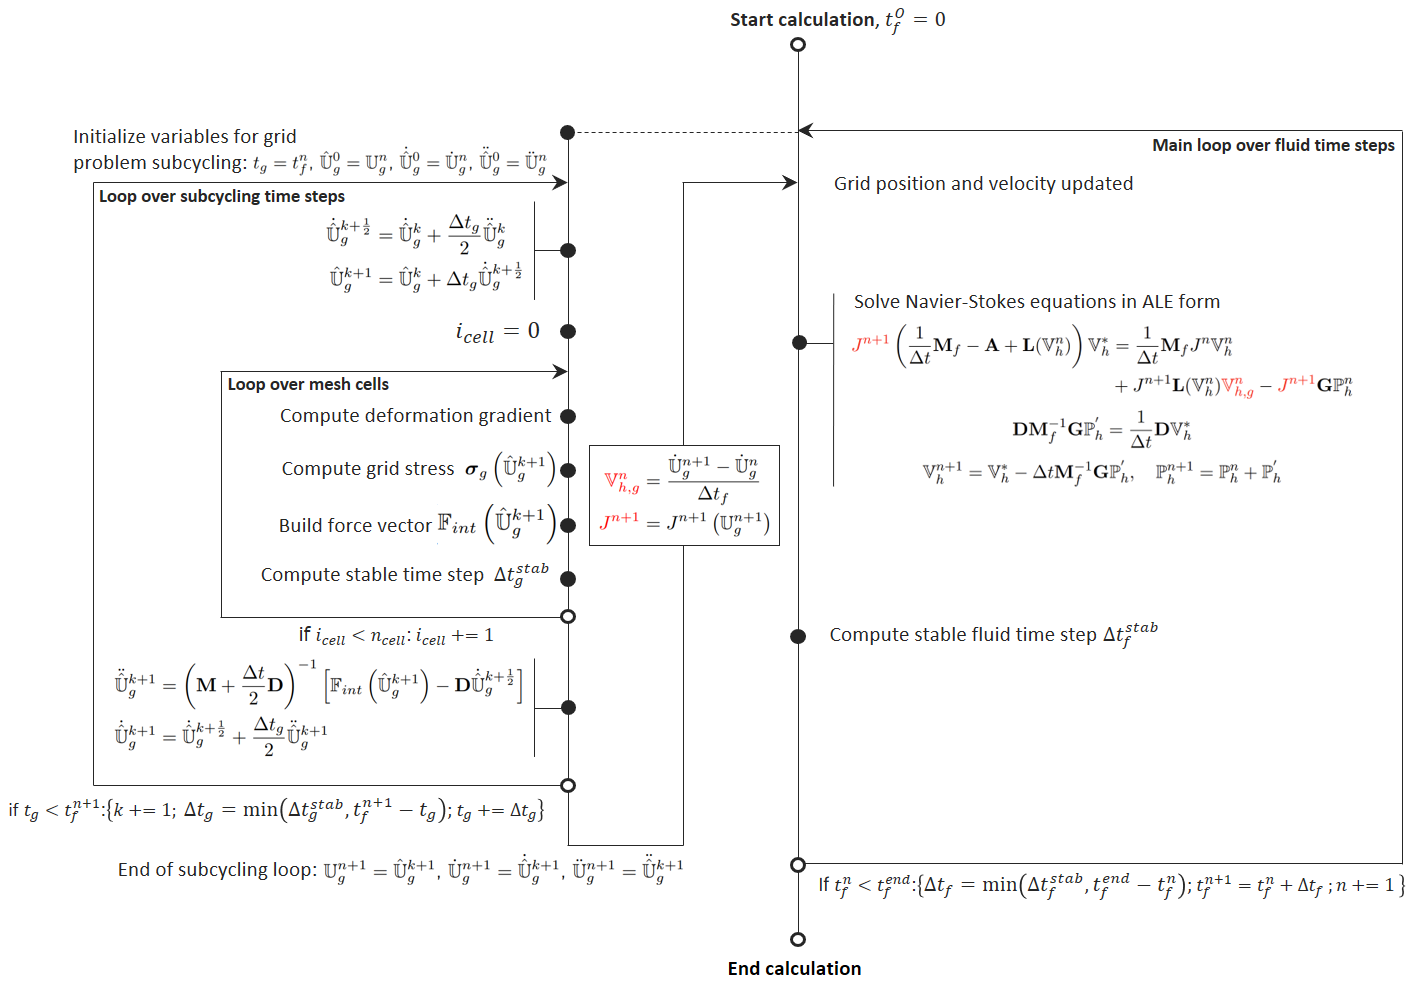
\includegraphics[scale=0.425]{figures/Grid_motion.png}
\caption{Complete algorithm for ALE Navier-Stokes solution with hyperbolic nonlinear problem for mesh motion.}
\label{fig:algorithm}
\end{figure}

\section{Optimized time step control}

Switching to an explicit solution of the hyperbolic grid problem, compared to the mandatory implicit solution of the initial elliptic problem, shifts the stakes for computational performance from the nonlinear system resolution to the control of the stable time step. Too small a time step, with respect to the stable time step of the fluid problem, will lead to an excessive number of subcycling iterations and counterbalance the benefit of the reduced cost of each iteration on the grid problem.

Some results on the highest time step ratio to preserve the computational competitiveness of the hyperbolic approach are available in \cite{leprevost_computationally_2023} for the simple case of the harmonic mesh model. A value below $200$ should be preferred, even though actual comparisons involving the computational cost of fully nonlinear models are challenging to obtain, and the benefit provided by explicit integration could be higher for complex cases. It is also noticeable that a minimum value of $10$ is advisable to obtain a quasi-static response of the grid to the imposed motion on Lagrangian boundaries from the perspective of the fluid solver. Such a ratio allows the waves to propagate in the domain and hides the dynamic nature of the hyperbolic equation.

The first action for time step control is in the choice of the fictitious material parameters, with the following priority order:

\begin{itemize}
    \item[$-$] first, set the parameters for the material behaviour: for instance, $E_g$ and $\nu_g$ in the case of the geometrically nonlinear Saint Venant-Kirchhof;
    \item[$-$] second, adjust the initial density $\rho_g$ of the fictitious grid material to set the speed of sound to the desired value, connected to the expected stable time step through the smallest characteristic length of all mesh cells: for the Saint Venant-Kirchhof model again, the speed of sound is uniform in space and easily obtained as $c = \sqrt{\frac{E_g}{\rho_g}}$.
\end{itemize}

Such a parameter analysis is of primary interest to gain knowledge on the full ALE system for the most robust and accurate simulation possible, involving the fluid solver with its stability conditions and the grid motion problem. However, it is insufficient to provide durable control over the time step ratio between the fluid problem and the grid problem. Two issues indeed remain:
\begin{enumerate}
    \item even for the simplest material models where the speed of sound is uniform in space and constant in time, the stable time step for the grid is still proportional to the smallest characteristic length of all mesh cells, which is likely to significantly decrease compared to the initial grid state in the case of large mesh motion ;
    \item more advanced material models than the Saint Venant-Kirchhof model are needed to handle very large imposed displacements on Lagrangian boundaries, such as nonlinear hyperelasticity, and in this case, the speed of sound is most of the time increasing with the level of stress, becoming non-uniform in space and non-constant in time (see Section \ref{sec-Mfront} for an example).
\end{enumerate}

The second action is thus the implementation into the explicit grid solver  a \textit{mass scaling} technique. Such methods are common in explicit structural dynamics software (see, for instance, LS-Dyna, Abaqus, or Radioss user manuals available online) to provide some control over the time step of the nonlinear simulations and satisfy the needs of engineering units. However, when implemented directly into a physical solver, they come with the risk of altering the solution of the problem of interest. Significant literature is available regarding the best ways to implement mass scaling safely in many cases. Some groundwork, as well as more recent work, can be found, for example, in~\cite{olovsson_selective_2005, stoter_critical_2023}, and a theoretical review is available in~\cite{voet_theoretical_2024}.

The management of the mesh motion problem in the present work is much easier regarding the usage of mass scaling than in the cases above since it does not directly influence the solution of the physical fluid problem. A straightforward and robust strategy can thus be safely implemented to provide the expected control over the grid stable time step. It expresses as follows, with a prescribed time step $\Delta t_g^p$ for the grid problem and for any mesh cell i where $\frac{l_i}{c_i} < \Delta t_g^p$: 
\begin{enumerate}
    \item compute the \textit{tangential} local Young's modulus $E_i^t$ such that $c_i = \sqrt{\frac{E_i^t}{\rho_i}}$, where $\rho_i$ is the local material density in cell $i$:
    
    \begin{equation}
      %\begin{aligned}
        \rho_i = \frac{\rho_g V_i^0}{V_i}, \quad 
        E_i^t = c_i^2 \rho_i,
      %\end{aligned}
    \end{equation}
    where $V_i$ is the current volume of cell $i$ and $V_i^0$ its initial value.
    
    \item compute the requested density $\rho_i^r$ to match the prescribed time step with the tangential Young's modulus:
    
    \begin{equation}
        \rho_i^r = E_i^t \left ( \frac{\Delta t_g^p}{l_i} \right )^2.
    \end{equation}
    
    \item compute the mass $\delta m_i$ to add to cell $i$ to match density $\rho_i^r$:
    
    \begin{equation}
        \delta m_i = V_i \rho_i^r - V_i \rho_i.
    \end{equation}
    
    \item equally distribute $\delta m_i$ among the nodes of cell $i$ and sum the result for each node and each space direction in the vector $\mathbf{M}_a$ of the same structure as the diagonal mass matrix $\mathbf{M}$.
\end{enumerate}




\section{Material models managed through MGIS/Mfront}
\label{sec-Mfront}
Solving efficiently, accurately, and robustly the behaviour of complex nonlinear material models in large strain formulation is the core thematic of an entire community (see, for instance, \cite{doghri_mechanics_2000, yavari_spatial_2006,blume_compatibility_1989}, among a rich literature, for generalities on nonlinear mechanics and specifics on large strain representation). As stated in the introduction, implementing advanced concepts from this field for the sole purpose of solving the ALE grid motion in a generic purpose CFD software is likely to be counterproductive in terms of skills management and code maintenance.

The \textbf{Mfront} open-source code-generation tool for material mechanics provides a very elegant alternative to this issue. It provides a \textit{Domain Specific Language} (DSL) allowing it to simply express any chosen constitutive relation. It then generates the corresponding source and compiles it into a dynamic library to be called each time the stress needs to be computed in the reference program of interest. The source code necessary for the proper calls to \textbf{Mfront}-built libraries is provided by the \textbf{MGIS} generic interface mentioned in the introduction and is the only building block for material mechanics to be implemented into the CFD software. The functions provided by \textbf{MGIS} very simply take as inputs the path to the material library, the values of the material parameters for the chosen model, including the density $\rho_g$, and the gradient of the transformation $\mathbf{F}$ at the evaluation point (see Section \ref{sec-elliptic-problems} for its expression with respect to the displacement field $\mathbf{u}_g$). They give as outputs, among many possibilities depending on the need, the Cauchy stress tensor $\boldsymbol{\sigma}_g$ and the speed of sound $c$.

Two material models are considered for testing purposes in the proposed work. First, the Saint Venant-Kirchhoff model. For illustration, the \textbf{Mfront} code for this model is given in Fig.~\ref{fig-code-mfront}. 
\begin{figure}[h]
\lstset{language=C++,
        basicstyle=\footnotesize,
        frame = single, 
        keywordstyle=\color{blue},
        stringstyle=\color{green},
        commentstyle=\color{green}\itshape,
        morecomment=[l][\color{magenta}]{\#},
        keywordsprefix=\@,alsoletter=\@
}
\begin{lstlisting}
@DSL DefaultFiniteStrainDSL;
@Behaviour SaintVenantKirchhoffElasticity;
@Author Thomas Helfer;
@Date 19/10/2013;
@Description{
  "The Saint Venant - Kirchhoff hyper elastic behaviour"
}

@ModellingHypotheses {".+"};

@MaterialProperty stress young;
@MaterialProperty real nu;
young.setEntryName("YoungModulus");
nu.setEntryName("PoissonRatio");

@LocalVariable stress lambda;   //<! First  Lame coefficient
@LocalVariable stress mu;       //<! Second Lame coefficient
@LocalVariable StrainStensor e; //<! Green-Lagrange strain

@InitLocalVariables{
  lambda = computeLambda(young,nu);
  mu     = computeMu(young,nu);
}

@Integrator{
  e = computeGreenLagrangeTensor(F1);
  const auto s = lambda*trace(e)*StrainStensor::Id()+2*mu*e;
  sig = convertSecondPiolaKirchhoffStressToCauchyStress(s,F1);
}

@SpeedOfSound{
  const auto jac = det(F1);
  v_sound=sqrt(abs(young)/(rho_m0*jac));
}
\end{lstlisting}
\caption{Mfront code for Saint Venant-Kirchhoff model.}
\label{fig-code-mfront}
\end{figure}

The second model is the Ogden hyperelastic model, selected for its capability to handle nearly incompressible materials with very large strain. This material model is defined through a decoupled potential $W$ decomposed into a volumetric part $W^v$ and an isochoric part $W^i$, such that:

\begin{equation}
    W(\mathbf{C}) = W^v(J) + W^i ( \lambda_1, \lambda_2, \lambda_3),
\end{equation}
with $\mathbf{C}$ the right Cauchy Green tensor: $\mathbf{C}=\mathbf{F}^T\mathbf{F}$, $J$ is the determinant of the deformation gradient: $J=\sqrt{det(\mathbf{C})}$, $\lambda_1$, $\lambda_2$, $\lambda_3$ are eigenvalues of $\mathbf{C}$. Both potentials are given by: 

\begin{equation}
  \label{eq-ogden-model}
  %\begin{aligned}
     W^v = \frac{1}{2}K (J - 1)^2 \quad \text{and} \quad 
     W^i = \displaystyle \sum_{p=1}^{N} \frac{\mu_p}{\alpha_p} \left ( \lambda_1^{\frac{\alpha_p}{2}} + \lambda_2^{\frac{\alpha_p}{2}} + \lambda_3^{\frac{\alpha_p}{2}} - 3 \right ),
  %\end{aligned}
\end{equation}
\noindent where $K, \left \{ \alpha_p \right \}_{p=1,N}, \left \{ \mu_p \right \}_{p=1,N}$ are material parameters.
The second Piola-Kirchhoff stress tensor is finally obtained as:

\begin{equation}
    \mathbf{S} = 2 \frac{\partial W^v}{\partial \mathbf{C}} + 2 \frac{\partial W^i}{\partial \mathbf{C}} = \mathbf{S}^v + \mathbf{S}^i.
\end{equation}

An example of user input is given in Fig.~\ref{fig-triocfd-mfront-data}, where the Ogden material model with $N=1$ is solved through the \underline{\textit{libBehaviour.so}} library whose absolute path is passed to the program. The entry names \underline{\textit{Ogden\_alpha}}, \underline{\textit{Ogden\_mu}}, and \underline{\textit{Ogden\_K}} map the material parameters $\alpha_1, \mu_1, K$ in eq.~(\ref{eq-ogden-model}), while \underline{\textit{Density}} and \underline{\textit{Inertial\_Damping}} provide the values for scalars $\rho_g$ and $d_g$ in eq.~(\ref{eq-final-grid-problem}). An implementation of the Ogden model is available in the \textbf{Mfront} gallery at \url{https://thelfer.github.io/tfel/web/ogden.html}.




\begin{figure}[H]
\lstset{language=C++,
        basicstyle=\footnotesize,
        frame = single
}
\begin{lstlisting}
Structural_dynamic_mesh_model dom
{
  Mfront_library {[local-absolute-path]}{/Ogden/src/libBehaviour.so}
  Mfront_model_name {Ogden}
  Mfront_material_property { {Ogden_alpha}   28.8 }
  Mfront_material_property { {Ogden_mu}   27778.  }
  Mfront_material_property { {Ogden_K} 69444444.  }
  Grid_dt_min 1.e-7
  Density 10000.
  Inertial_Damping 1000.
}
\end{lstlisting}
\caption{Example of input data for usage of \textbf{Mfront} library for grid mesh motion.}
\label{fig-triocfd-mfront-data}
\end{figure}

\chapter{Partitioned coupling between Euler-Bernoulli beams and incompressible viscous Newtonian fluids}



The high computational resources required for FSI simulations can be a limitation for industrial
applications. To address this, a one-dimensional Euler-Bernoulli beam model is proposed as a
simplified modeling approach for slender structures. The beam model is integrated into TrioCFD, enabling internal fluid-structure coupling and reducing data exchange between separate
software. 
By embedding the
structural model directly within the CFD code, the approach eliminates the need for traditional code-to-code coupling, providing a
simpler and more efficient FSI framework. This approach eliminates the need for inter-solver coupling, three-dimensional interpolations, data exchange, and communication between separate
solvers. The solid solver employs an unconditionally stable time
discretization scheme that only requires the solution of diagonal
matrix systems, ensuring numerical robustness and computational
efficiency. The time coupling for FSI follows the explicit conventional serial staggered (CSS) algorithm.

The fluid-structure coupling strategy follows a partitioned approach, where the fluid and solid problems are solved independently by their respective solvers. The coupled system is iteratively solved at each time step, where variables are exchanged at the fluid-structure interface. This approach allows the use of distinct mathematical models, numerical methods, and discretization techniques for each medium. In this work, the fluid dynamics are solved using the incompressible fluid module of TrioCFD while the structure is modeled using the new beam module of TrioCFD.  The coupling is performed through boundary conditions at the fluid-structure interface, ensuring the continuity of the velocities and the normal component of the stress tensors. Denoting \({\Gamma}_{FS}\) as the set of all time-dependent moving interfaces (which reduces to $\partial\mathcal{C}$) that can exist in a fluid-structure problem, the boundary conditions can be written as
\begin{subequations}\label{eq:BC_on_IFS}
  \begin{align}
  \label{eq:BC_Dirichlet}
{\mathbf{V}} - \frac{\partial{{\mathbf{U}}}}{\partial T}&={\mathbf{0}},\quad \text{on}\quad  {\Gamma}_{FS},\\  
\label{eq:BC_Neumann}
\left({\boldsymbol{\sigma}}_{f} -{\boldsymbol{\sigma}}_{s}\right)\cdot {\mathbf{n}}_{sf}&= {\mathbf{0}},\quad \text{on}\quad  {\Gamma}_{FS},
\end{align}
\end{subequations} 
where \(\mathbf{V}\), \({\boldsymbol{\sigma}}_{f}\), \(\partial {\mathbf{U}}/\partial T\), and \({\boldsymbol{\sigma}}_{s}\) represent the velocity, stress tensor for the fluid, velocity, stress tensor for the structure, respectively. The vector \({\mathbf{n}}_{sf}\) represents the unit normal vector of the interface ${\Gamma}_{FS}$, oriented from the structure to the fluid. 
At each time iteration, the Navier-Stokes equations are solved for the variables \(({\mathbf{V}}, P)\), subject to Dirichlet boundary conditions \eqref{eq:BC_Dirichlet} on \(\Gamma_{FS}\), while the structure equation~\eqref{Eq_EulerBernoulli} is solved with Neumann boundary conditions \eqref{eq:BC_Neumann} on \(\Gamma_{FS}\).

\section{Euler-Bernoulli beam model with modal resolution}

The dynamics of the structure, here after denoted by ${\mathcal{C}}$,  is modeled by an Euler-Bernoulli beam equation, including mass and stiffness proportional Rayleigh damping coefficients, $\alpha_1$ and $\alpha_2$, respectively. This equation can be written as
\begin{equation}
\label{Eq_EulerBernoulli}
\rho_{s} S_{} \frac{\partial^{2} Y_{}}{\partial T^{2}}+\frac{\partial}{\partial T}\left(2\alpha_1 \rho_{s} S_{} Y_{}+2\alpha_2 E_{} I_{} \frac{\partial^{4} Y_{}}{\partial {X_1}^{4}}\right)+E_{} I_{} \frac{\partial^{4} Y_{}}{\partial {X_1}^{4}}= \overline{F}.
\end{equation}

The term $\overline{F_{}}$ in Eq. \eqref{Eq_EulerBernoulli} represents the $\boldsymbol{\mathrm{e}}_{2}$-component of the linear fluid force on $\mathcal{C}_{}$ due to its own motion.

The modal representation of the Euler-Bernoulli beam equation \eqref{Eq_EulerBernoulli} is obtained by expressing the neutral axis displacement as a linear expansion
\begin{equation}\label{Eq_Expansion_Displacement_Modal}
Y\left(X_1,T\right) = \sum_{k=1}^{m} Q^{(k)}(T) \frac{W^{(k)}(X_1)}{N^{(k)}},
\end{equation}
where \( Q^{(k)}(T) \) represents the time-dependent dimensional amplitude of the \( k \)-th structural vibration mode of the beam, denoted by \( W^{(k)}(X) \).
Substituting Eq.~\eqref{Eq_Expansion_Displacement_Modal} into Eq.~\eqref{Eq_EulerBernoulli} and projecting onto the structural vibration mode \( W^{(l)} \), for \( l \in \llbracket 1,m\rrbracket \), leads to the modal equation
\begin{equation}
\label{eq:eq_poutre_mode_vect_damping}
[\mathbf{M}] \ddot{\mathbf{Q}} + [\mathbf{C}] \dot{\mathbf{Q}} + [\mathbf{K}] {\mathbf{Q}} = {\mathbf{F}},
\end{equation}
where \(\mathbf{Q}\) is the real column vector of length \(m\) containing the modal amplitudes \( Q^{(k)} \). The terms \(\ddot{\mathbf{Q}} = {\textrm{d}}^2{\mathbf{Q}}/{\textrm{d}}T^2\) and \(\dot{\mathbf{Q}} = {\textrm{d}}{\mathbf{Q}}/{\textrm{d}}T\) denote the second and first time derivatives of \(\mathbf{Q}\), respectively.
In Eq.~\eqref{eq:eq_poutre_mode_vect_damping}, the right-hand side term \({\mathbf{F}}\) represents the time-dependent modal dimensional linear fluid force. It is a vector of length \(m\), whose \(k\)-th element is given by  
$F^{(k)} = \left\langle W^{(k)},\overline{F} \right\rangle_{L}/N^{(k)}$. In Eq.~\eqref{eq:eq_poutre_mode_vect_damping}, $[\mathbf{M}]$, $[\mathbf{C}]$, and $[\mathbf{K}]$ are the dimensional structural mass, damping, and stiffness modal matrices. These matrices, of size $m\times m$, are diagonal due to the orthogonality of the modes, with diagonal terms 
\begin{subequations}
\begin{align}
         M^{(kk)} &= \rho_s S \frac{\left\langle W_{}^{(k)},W_{}^{(k)}\right\rangle_{L}}{N_{}^{(k)}N_{}^{(k)}},\\
         C^{(kk)} &= 2 \left(\alpha_1 \rho_s S + \alpha_2 EI \left(\frac{\lambda^{(k)}}{L}\right)^4\right)\frac{\left\langle W_{}^{(k)},W_{}^{(k)}\right\rangle_{L}}{N_{}^{(k)}N_{}^{(k)}},\\
         K^{(kk)} &= EI \left(\frac{\lambda^{(k)}}{L}\right)^4 \frac{\left\langle W_{}^{(k)},W_{}^{(k)}\right\rangle_{L}}{N_{}^{(k)}N_{}^{(k)}}.
\end{align}
\end{subequations}
Equation \eqref{eq:eq_poutre_mode_vect_damping} is time-discretized using the Hilbert-Hughes-Taylor (HHT) scheme, also known as the HHT-\(\alpha\) method, see~\cite{HHT} for more details. Denote \(\Q^{n}\), \(\dot{\Q}^{n}\), \(\ddot{\Q}^{n}\) and ${\mathbf{F}}^{n}$ as the values of \(\Q\), \(\dot{\Q}\), \(\ddot{\Q}\) and ${\mathbf{F}}$, respectively, at the time instant \(T^{n} = n \Delta T\), $n\in\llbracket 0,n_{max}\rrbracket$. The HHT scheme can then be written as
\begin{subequations}\label{eq:HHT}
 \begin{align}
 &\left( [\mathbf{M}] + \gamma \Delta T (1+\alpha) [\mathbf{C}] + \beta \Delta T^2(1+\alpha) [\mathbf{K}] \right) \ddot{\Q}^{n+1} = (1+\alpha){\mathbf{F}}^{n+1} -\alpha {\mathbf{F}}^{n} \nonumber\\
 & \quad \quad \quad \quad \quad   \quad \quad \quad\quad \quad \quad \quad \quad \quad \quad \quad \quad \quad \quad \quad  \quad \quad - (1+\alpha) [\mathbf{C}] \left( \dot{\Q}^{n} + (1-\gamma)\Delta T \ddot{\Q}^{n} \right)\nonumber \\
 & \quad \quad \quad \quad \quad   \quad \quad \quad\quad \quad \quad \quad \quad \quad \quad \quad \quad \quad \quad \quad \quad \quad  - (1+\alpha) [\mathbf{K}]\left( \Q^{n} + \Delta T \dot{\Q}^{n} + \Delta T^2 \left( \frac{1}{2}- \beta\right) \ddot{\Q}^{n}\right)\nonumber\\ &\quad \quad \quad \quad \quad \quad \quad \quad \quad  \quad \quad \quad\quad \quad \quad \ \quad \quad \quad \quad \quad  \quad \quad + \alpha [\mathbf{C}]  \dot{\Q}^{n} + \alpha [\mathbf{K}]  \Q^{n},\label{eq:HHT_a} \\
&\dot{\Q}^{n+1} = \dot{\Q}^{n} + (1-\gamma) \Delta T \ddot{\Q}^{n} + \gamma \Delta T \ddot{\Q}^{n+1},\label{eq:HHT_b} \\
&\Q^{n+1} =  \Q^{n} +  \Delta T \dot{\Q}^{n} + \Delta T^2 \left( \frac{1}{2}- \beta\right) \ddot{\Q}^{n} +  \Delta T^2 \beta \ddot{\Q}^{n+1}.\label{eq:HHT_c}
\end{align}
\end{subequations}
In Eq. \eqref{eq:HHT}, the parameters $\alpha$, $\beta$, and $\gamma$ are typically chosen as \(\alpha \in [-1/3, 0]\), \(\beta = (1 - \alpha)^2 / 4\), and \(\gamma = 1/2 - \alpha\), which ensures that the scheme is unconditionally stable. The parameter \(\alpha\) introduces dissipation for high frequencies. Specifically, \(\alpha = 0\) corresponds to the Newmark average acceleration integration scheme~\cite{newmark1959method}.

Starting from an initial state \(\left({\Q}^{0},\dot{\Q}^{0}\right)\), the quantities \(\ddot{\Q}^{n}\), \(\dot{\Q}^{n}\), and \({\Q}^{n}\) are successively determined using Eqs. \eqref{eq:HHT_a}, \eqref{eq:HHT_b}, and \eqref{eq:HHT_c}, respectively.  
The quantity \(\dot{\Q}^{n}\) is then used to determine the velocity of the neutral axis of the beam, which according to Eq. \eqref{Eq_Expansion_Displacement_Modal} is
\begin{equation}
    \forall n\in\llbracket 1,n_{max}\rrbracket,\quad \dot{Y}^{n} (X_1)=\sum_{k=1}^m \dot{Q}^{(k), n}  \frac{W^{(k)} (X_1)}{N^{(k)}}.
\end{equation}
In the general case of flexural motions about the \(\boldsymbol{\mathrm{e}}_{2}\) and \(\boldsymbol{\mathrm{e}}_{3}\) directions, the three-dimensional velocity \(\dot{\mathbf{U}}^{n}\) of a point \((X_1, X_2, X_3)\in\Gamma_{FS}\) is defined by the Euler-Bernoulli kinematic relation
\begin{align}\label{3d_modal_def}
    \forall n\in\llbracket 1,n_{max}\rrbracket,\quad \dot{\mathbf{U}}^{n}(X_1, X_2, X_3) = &\sum_{k=1}^{m} \dot{Q}^{(k),n}_Y \frac{1}{N_{Y}^{(k)}}\left(- X_2 \frac{{\textrm{d}} W_Y^{(k)}}{{\textrm{d}} X_1}(X_1) \boldsymbol{\mathrm{e}}_{1} +  W_Y^{(k)}(X_1) \boldsymbol{\mathrm{e}}_{2} \right)\nonumber\\
+ &\sum_{k=1}^{m} \dot{Q}^{(k),n}_Z \frac{1}{N_{Z}^{(k)}}\left( X_3 \frac{{\textrm{d}} W_Z^{(k)}}{{\textrm{d}} X_1}(X_1) \boldsymbol{\mathrm{e}}_{1} +  W_Z^{(k)}(X_1) \boldsymbol{\mathrm{e}}_{3} \right),
\end{align}
where $\dot{Q}^{(k),n}_Y$ (resp. $\dot{Q}^{(k),n}_Z$) is the modal velocity of the structural vibration mode $W_Y^{(k)}$ (resp. $W_Z^{(k)}$) of infinity norm $N_Y^{(k)}$ (resp. $N_Z^{(k)}$). The modal velocity $\dot{Q}^{(k),n}_Y$ can be calculated from Eq. \eqref{eq:HHT}, considering ${\mathbf{F}}^{n}$ as the vector containing the modal fluid forces $F^{(k),n}_Y$. These modal forces are given by    
\begin{equation}
      \forall \left(k,n\right)\in\llbracket 1,m\rrbracket\times\llbracket 1,n_{max}\rrbracket,\quad    F^{(k),n}_Y= \boldsymbol{\mathrm{e}}_2\cdot\int_{\Gamma_{FS}} \left(-P^n \mathbf{n}_{sf}  +\rho_f \nu_f  \left[\nabla {{\mathbf{V}}^n} +\left(\nabla {{\mathbf{V}}^n} \right)^{T} \right]\cdot \mathbf{n}_{sf} \right) \frac{{W}^{(k)}_Y}{{N_{Y}^{(k)}}}{\textrm{d}}S,
     \label{eq:_modal_force_Y}
    \end{equation}
where $\left(\nabla{{\mathbf{V}}} \right)^{T}$ is the transpose of the velocity gradient tensor $\nabla{{\mathbf{V}}}$ and ${\textrm{d}}S$ is an infinitesimal surface element of $\Gamma_{FS}$. 
 The calculation of \( F^{(k),n}_Z \) follows similarly, replacing \( \boldsymbol{\mathrm{e}}_2 \) and \( W_Y^{(k)} \) with \( \boldsymbol{\mathrm{e}}_3 \) and \( W_Z^{(k)} \), respectively, in Eq.~\eqref{eq:_modal_force_Y}.
In Eq. \eqref{3d_modal_def}, the terms \(- X_2 {{\textrm{d}} W_Y^{(k)}}/{{\textrm{d}} X_1}\) and  \(X_3 {{\textrm{d}} W_Z^{(k)}}/{{\textrm{d}} X_1}\) represent the axial displacement component in the \(\boldsymbol{\mathrm{e}}_1\)-direction, which arises due to the rotation of the cross-sections. Further details can be found in~\cite{lagrange2025fluid}.


\section{Coupling algorithm}\label{sec:CSS}

In this work, the explicit Conventional Serial Staggered (CSS) algorithm (see~\cite{CSS} for more details) is used to couple the fluid and the structure. The CSS algorithm, illustrated in Fig.~\ref{explicite}, proceeds as follows. At time \(T^n\), $n>0$, the structure velocity \(\dot{\mathbf{U}}^{n}\), the fluid velocity \(\V^{n}\), and the fluid pressure \(P^{n}\) are known. To advance to the next time step \(T^{n+1}\), the following sequence is performed:
\begin{enumerate}
    \item The structure velocity $\dot{\mathbf{U}}^{n}$ is communicated to the fluid solver through the coupling interface. 
    \item The grid velocity $\V^{n+1}_{h,ALE}$ is determined using Eq.~\eqref{harmonic_mesh}, with $\mathbf{v}_{S} = \dot{\mathbf{U}}^{n}$ in Eq.~\eqref{harmonic_mesh}. {The position vector ${\mathbf{X}}^n$ of a point on the grid is updated according to
 ${\mathbf{X}}^{n+1} = {\mathbf{X}}^{n} + \Delta T \V^{n+1}_{h,ALE}$.}
    \item Equation \eqref{eq:NS_ALE2} is solved for \(\V^{n+1}\) and \(P^{n+1}\), using the boundary condition \(\dot{\mathbf{U}} = \dot{\mathbf{U}}^{n}\).  
    \item The modal fluid forces $F^{(k), n+1}$ are computed using the fluid velocity $\V^{n+1}$ and pressure $P^{n+1}$, according to Eq.~\eqref{eq:_modal_force_Y}. The computed forces are then transferred to the structure solver through the coupling interface.
    \item The quantities \(\ddot{\Q}^{n+1}\), \(\dot{\Q}^{n+1}\) and \({\Q}^{n+1}\) are computed using Eqs. \eqref{eq:HHT_a}, \eqref{eq:HHT_b} and \eqref{eq:HHT_c}, respectively.
    \item The structure velocity $\dot{\mathbf{U}}^{n+1}$ is reconstructed according to Eq. \eqref{3d_modal_def}.
    \item If \(T^{n+1}\) reaches the final time, the process stops. Otherwise, the time loop advances to \(T^{n+2} = T^{n+1} + \Delta T\), using a time step \(\Delta T\) that satisfies the fluid CFL condition. The solid discretization imposes no restrictions on the time step, as the HHT scheme is unconditionally stable.  Further details can be found in~\cite{lagrange2025fluid}.
\end{enumerate}

\begin{figure}[h!]
  \centering
  \resizebox{1.\textwidth}{!}{
    \begin{tikzpicture}
      \centering 
      \draw (0,0.5) node[anchor=north,rounded
      corners=3pt,draw=blue]{FLUID};
      \draw (8,0.5) node[anchor=north,rounded
      corners=3pt,draw=green]{STRUCTURE};
      \draw (4,0.5) node[anchor=north,rounded
      corners=3pt,draw=red]{COUPLING};
      %\draw[-latex] (0,-1) -- (0,-4.1);

      \draw (0,-1) node[anchor=north,rounded
      corners=3pt,draw=blue,fill=white]{$\V^{n}, P^{n}$};  
      \draw (6,-2.) node[anchor=east]{
        \begin{minipage}{4.5cm}
           \circled{1} Send structure velocity \color{red}$\dot{\mathbf{U}}^{n}$
         
        \end{minipage}}; 
      \draw (8,-2) node[anchor=north,rounded
      corners=3pt,draw=green,fill=white]{$\ddot{\Q}^{n}, \dot{\Q}^{n}, \Q^{n}$};
      %\draw[-latex] (0,-3.4) -- (0,-5.);
      \draw[-latex, blue] (0.,-1.5) -- (0.,-4.);
      %\draw[-latex] (0,-3.4) -- (1.9,-4.1);
%      \draw (0,-3.4) node[anchor=north,rounded
%      corners=3pt,draw=black,fill=white]{
%      $\vect{F}_{I,i}^{n}$,
%        $\vect{\mathcal{M}}_{I,i}^{n}$}; 
      \draw[-latex, red] (6.9,-2.25) -- (0.,-2.25);
 


      \draw[-latex, green] (8,-2.5) -- (8,-5.5); 
      \draw (7.95,-5) node[anchor=west]{
        \begin{minipage}{3cm}
         \circledg{4} Struct. update
        \end{minipage}};

      
      \draw (0.9,-2.8) node[anchor=east]{
        \begin{minipage}{4cm}
          \circledb{2} Fluid update
        \end{minipage}};

      \draw[-latex, red] (0.9,-4.35) -- (8,-4.35);
      
      \draw (7.,-5) node[anchor=south east]{
        \begin{minipage}{5.cm}
          \circled{3} Send fluid force \color{red}$\F^{n+1}$
           
            
      \end{minipage}};
      \draw (0.,-4.) node[anchor=north,rounded
      corners=3pt,draw=blue,fill=white]{$\V^{n+1}, P^{n+1}$};
      \draw (8,-5.5) node[anchor=north,rounded
      corners=3pt,draw=green,fill=white]{$\ddot{\Q}^{n+1}, \dot{\Q}^{n+1}, \Q^{n+1}$}; 
    \end{tikzpicture}
  }
  \caption{Sketch of the explicit Conventional
Serial Staggered algorithm. First, the structure velocity \(\dot{\mathbf{U}}^{n}\) is sent to the fluid solver. Second, it is used to compute the fluid velocity $\V^{n+1}$ and pressure $P^{n+1}$. Third, the resulting modal fluid force ${\mathbf{F}}^{n+1}$ is transferred to the structure solver. Fourth, ${\mathbf{F}}^{n+1}$ is used to compute the modal displacement $\Q^{n+1}$, velocity $\dot{\Q}^{n+1}$, and acceleration $\ddot{\Q}^{n+1}$.  
}
  \label{explicite}
\end{figure}



\section{Euler--Bernoulli Beam Model Configuration}

This section describes how to configure an Euler--Bernoulli beam model inside
the \texttt{Beam\_model} block of a TrioCFD input file.
The formulation supports vibrations in one or two bending planes as well as an
arbitrary orientation of the beam in space.  
For each beam, the user must provide modal data (mass, stiffness, mode shapes,
abscissae, initial conditions) and specify the geometric and numerical
parameters of the model.

\subsection*{General Structure}

A typical \texttt{Beam\_model} block contains the definition of one or several
beams, each introduced with a \texttt{Name} section.  
The global structure is:

\begin{lstlisting}
Beam_model my_domain
{
    nb_beam <number_of_beams>

    Name <beam_name> {
        ... beam configuration ...
    }

    Name <beam_name> {
        ... beam configuration ...
    }
}
\end{lstlisting}

\subsection*{Description of User Parameters}

Each beam requires the following fields:

\begin{itemize}
  \item \texttt{nb\_planes}: number of bending planes (1 or 2).
  \item \texttt{nb\_modes}: number of structural vibration modes to load.  If multiple planes are used (\texttt{nb\_planes > 1}),  the modes are divided evenly across planes. 
  \item \texttt{longitudinal\_axis}: main axis of the beam (x, y, or z).
  \item \texttt{bendingDirection}: bending direction for the beam:
\begin{itemize}
    \item Single-plane (\texttt{nb\_planes = 1}): User must provide the bending direction explicitly.
    \item Two-plane (\texttt{nb\_planes = 2}): 
        \begin{itemize}
            \item User provides only the first plane direction.
            \item Second plane direction is determined automatically as perpendicular to both the beam axis and the first bending direction.
        \end{itemize}
\end{itemize}
  \item \texttt{BaseCenterCoordinates}: 3D coordinates of the beam axis origin.
  \item \texttt{NewmarkTimeScheme}: MA (Newmark mean acceleration) or HHT (Hilber-Hughes-Taylor) numerical scheme parameters.
  \item \texttt{Mass\_and\_stiffness\_file\_name}: modal mass and stiffness data. Must contain exactly \texttt{nb\_modes} lines.
  \item \texttt{Absc\_file\_name}: 1D abscissae of the modal deformation.
  \item \texttt{CI\_file\_name}: initial modal state (displacement). Must contain exactly \texttt{nb\_modes} lines.
  \item \texttt{Modal\_deformation\_file\_name}: one file per mode, each must contain exactly two numerical columns:\\
        \quad (1) the modal deformation \(W(X)\)\\
        \quad (2) its derivative \(-\mathrm{d}W/\mathrm{d}X\) (cross-section rotation)

The number of rows must match the abscissae provided in \texttt{Absc\_file\_name}.

  \item \texttt{Output\_position\_1D}: locations along the beam axis for 1D output.
  \item \texttt{Output\_position\_3D}: 3D coordinates of points where the full
        3D beam displacement is interpolated and output.
\end{itemize}



\subsection*{Complete Example}

Below is a complete example with two beams, each vibrating in two bending planes.


\begin{lstlisting}
Beam_model dom_cylindres
{
    nb_beam 2

    Name cylindre1 {
        nb_modes 20
        longitudinal_axis z       
        bendingDirection x      
        nb_planes 2

        BaseCenterCoordinates 0.0035 0. 0.
        NewmarkTimeScheme HHT -0.1

        Mass_and_stiffness_file_name ../Cylindre1/vibr_pout2tube.txt
        Absc_file_name ../Cylindre1/vibr_pout2tube_absc.txt
        CI_file_name ../Cylindre1/vibr_pout2tube_CI.txt

        Modal_deformation_file_name 20 \
            ../Cylindre1/phi_1.txt ../Cylindre1/phi_2.txt ...

        Output_position_1D 1 50
        Output_position_3D 1 0.007 0.0035 0.198
        
        # Restart_file_name cylindre1SaveBeamForRestart.txt #  # Optional: file to resume calculations #

    }

    Name cylindre2 {
        nb_modes 20
        longitudinal_axis z
        bendingDirection x
        nb_planes 2

        BaseCenterCoordinates 0.0485 0. 0.
        NewmarkTimeScheme HHT -0.1

        Mass_and_stiffness_file_name ../Cylindre2/vibr_pout2tube.txt
        Absc_file_name ../Cylindre2/vibr_pout2tube_absc.txt
        CI_file_name ../Cylindre2/vibr_pout2tube_CI.txt

        Modal_deformation_file_name 20 \
            ../Cylindre2/phi_1.txt ../Cylindre2/phi_2.txt ...

        Output_position_1D 1 50
        Output_position_3D 1 0.052 0.0035 0.198
        
        # Restart_file_name cylindre2SaveBeamForRestart.txt #  # Optional: file to resume calculations #
    }
}
\end{lstlisting}


\begin{figure}[h!]
\centering
\begin{tikzpicture}[scale=3.5,>=stealth]

% Draw beam axis
\draw[thick, ->] (0,0,0) -- (3,0,0) node[anchor=north] {$e_\text{long}$};

% Draw local coordinate frame at the start
\draw[->, red] (0,0,0) -- (0,0.8,0) node[left] {$e_\text{trans,1}$};
\draw[->, blue] (0,0,0) -- (0,0,0.8) node[right] {$e_\text{trans,2}$};

% Draw transverse displacement W in plane 1 (red)
\draw[red, thick, ->] (1,0,0) -- (1,0.4,0) node[midway, left] {$W_1$};

% Draw transverse displacement W in plane 2 (blue)
\draw[blue, thick, ->] (2,0,0) -- (2,0,0.4) node[midway, right] {$W_2$};

% Draw rotation vectors (R) as small arcs
\draw[red, ->] (1,0.4,0) arc (90:120:0.15);
\draw[blue, ->] (2,0,0.4) arc (0:30:0.15);

% Label beam ends
\node at (0, -0.2,0) {Beam Base};
\node at (3, -0.2,0) {Beam Tip};

\end{tikzpicture}
\caption{Euler-Bernoulli beam with two bending planes. $e_\text{long}$ is the beam axis, $e_\text{trans,1}$ and $e_\text{trans,2}$ are bending directions. $W_1, W_2$ are transverse displacements.}
\end{figure}
